\documentclass[aps, prc, reprint, amsmath, groupedaddress, nofootinbib]{revtex4-1}
\usepackage[compat=1.1.0]{tikz-feynman}
\usepackage[utf8]{inputenc}
\usepackage{hyperref}
\usepackage{amsmath}
\usepackage{amssymb}
\usepackage{amsfonts}
\usepackage{tabularx}
\usepackage{booktabs}
\usepackage{graphicx}
\usepackage{color}
\usepackage{multirow}
\usepackage[inline]{enumitem}
\graphicspath{{fig/}}
\definecolor{theblue}{RGB}{0,50,230}
\usepackage{appendix}
\hypersetup{
  colorlinks=true,
  linkcolor=theblue,
  citecolor=theblue,
  urlcolor=theblue
} 



\newcommand{\trento}{T\raisebox{-0.5ex}{R}ENTo}
\newcommand{\nch}{N_\text{ch}}
\newcommand{\sqrts}{\sqrt{s_{NN}}}
\newcommand{\T}{\tilde{T}}
\newcommand{\paddedhline}{\noalign{\smallskip}\hline\noalign{\smallskip}}
\newcommand{\dnchdy}{dN_\text{ch}/d\eta}
\newcommand{\dndypP}{dN_\text{pPb}/d\eta}
\newcommand{\dndyPP}{dN_\text{PbPb}/d\eta}
\newcommand{\x}{\mathbf x}
\newcommand{\y}{\mathbf y}
\newcommand{\z}{\mathbf z}
\newcommand{\trans}{^\intercal}

\newcommand{\Raa}{R_{AA}}
\newcommand{\vv}{v_2\{2\}}
\newcommand{\vvv}{v_3\{2\}}
\newcommand{\vnv}{v_n\{2\}}
\newcommand{\ppi}{\frac{\partial}{\partial p_i}}
\newcommand{\ppj}{\frac{\partial}{\partial p_j}}
\newcommand{\ppl}{\frac{\partial}{\partial p_l}}
\newcommand{\Kpara}{\kappa_{\|}}
\newcommand{\Kperp}{\kappa_{\perp}}
\newcommand{\Ppara}{\hat{P}^{\|}}
\newcommand{\Pperp}{\hat{P}^{\perp}}

\begin{abstract}
Current observation of open charm in heavy-ion collisions shows unexpectedly large momentum anisotropy and small nuclear modification factor, posing a challenge to the theoretical understanding of the nature of coupling between heavy quark and the medium.
Linear Boltzmann transport and Langevin diffusion are two popular kinetic models for heavy quark in-medium propagation.
In this work, we develop a hybrid heavy quark transport model that combines the strengths of both: 
heavy quarks are evolved with Langevin diffusion using an empirical diffusion constant and scattering processes treated linear Boltzmann equations with perturbative matrix elements.
The Langevin component is a complementary contribution to the linear Boltzmann equation when perturbative scattering is inadequate.
Both elastic and inelastic scatterings are included in the Boltzmann component.
The Landau-Pomeranchuk-Migdal effect is treated effectively via gluon formation time and detailed balance is imposed between gluon emission and absorption.
With the hybrid model, we study the heavy flavor momentum anisotropic, nuclear modification factor, and correlation observables in A-A collisions at the RHIC and the LHC energies.
Comparing to available D and B meson data, we constrain the diffusion constant of the Langevin component.

\end{abstract}


\begin{document}


\title{A hybrid heavy quark transport model in a quark-gluon plasma that couples linear Boltzmann equation and Langevin diffusion dynamics}
\author{Weiyao Ke}
\author{Yingru Xu}
\author{Steffen A.\ Bass}
\affiliation{Department of Physics, Duke University, Durham, NC 27708-0305}
\date{\today}
\maketitle

\section{Introduction}
In recent years, Relativistic Heavy-Ion Collider (RHIC) at Brookhaven National Laboratory and later the Large Hadron Collider (LHC) at CERN discovered a new state of matter, namely the strongly coupled quark-gluon plasma (sQGP), in ultra-relativistic heavy-ion collisions.
Two key signatures in the discoveries of sQGP are the collective flows and the jet quenching.
The collective flows reveal the surprising fact that the bulk medium of sQGP undergoes a strong collective expansion after being produced and the behaviors can be explained in great details by viscous hydrodynamics with the smallest specific viscosity ($\eta/s$) ever discovered in nature.
The jet quenching refers to that the yield of high transverse momentum hadrons in nuclear collisions are strongly suppressed compared to the yield in proton proton collision where medium effects should be small.
Calculations have shown that this suppression is a consequences of jet losing energy to the hot, dense and color-deconfined medium. 

Open heavy flavors (charm and bottom) as probes of sQGP partly belong to the jet observables but they are also unique because of the large masses and flavors.
Since the temperatures achieved in the experiments are still much smaller than charm and bottom masses, their thermal productions are highly suppressed; 
therefore the dominant production mechanism is production through initial hard process.
Heavy flavors are rare in heavy ion collisions even at low transverse momentum due to the mass, so they barely annihilate or recombine with their anti-particles, roughly conserving its number during the time-scale of sQGP.
These two features are particular attractive to theorists as heavy quarks experienced the medium full-time evolution and flavor-tagged particles are much easier to track in the calculations than the evolution of a full jet.
Finally, the mass sets an additional energy scale to the problem and brings rich physics to the heavy flavor sector.
In the high transverse momentum region, heavy quarks lose energy mainly through radiative process and this merge into the regime of jet energy loss study;
in the low momentum region, mass effect delays its thermalization time, providing a window to study the equilibration process.
Heavy flavors are therefore an ideal and unique probe to study the sQGP properties.

The in-medium propagation of heavy flavors is often studied in a kinetic approach that is linearized with respect to heavy quark distribution function. 
This linearization means any back reactions from heavy quark to the medium are neglected.
Linearized Boltzmann transport equation and Langevin equation are both widely used linearized models but focus on different levels of description of the interaction.
The linearized Boltzmsport equation is built on elementary scattering processes that can be directly related to fundamental calculations.
In principal, perturbative-QCD (pQCD) can predict the cross-section of these elementary scatterings.
However, these calculation in the presence of a medium is extremely complicated even at leading order.
Also, the pQCD processes are often plagued by soft divergence that need to be regulated by a medium scale proportional to the temperature, but with current collision energies the relevent temperature scale is not high enough that brings large ambiguity to pQCD calculation through the scale dependence of the strong coupling constant $\alpha_s(\mu T)$.
The Langevin equation takes a different perspective. 
It assumes that heavy quark receives frequent but soft momentum kicks from the medium, then a statistical description in terms of "drag" and "diffusion" coefficients of the interaction is possible.
These transport coefficients encode the first and second momentums of the momentum exchange rate but are agnostic to further details of the elementary processes.
One can again evaluate these transport coefficients from first principals, but for us focusing on learning these properties from experiment data, it is the vast flexibility to parametrize these quantities that the Langevin equation is most useful.
Of course, in this way it is not clear how to establish a direct relation between the extracted values and a more fundamental understanding.
In this work, we would like to combine the strengths of both approaches
and we have developed a hybrid heavy quark transport model described as follows.
The heavy quark scatters off medium particles in a linear Boltzmann equations with pQCD matrix elements (the scattering component), and between scatterings heavy quark is propagated by a Langevin equation (the diffusion component) with empirical transport coefficient mimicing the interaction missing from the above scattering picture.
Both elastic and inelastic scatterings are included in the scattering component with soft divergence screened by a Debye mass $m_D^2 \sim \alpha_s T^2$ and Landau-Pomeranchuk-Migdal (LPM) effect taken into account effectively.
The renormalization scale $\mu$ is the only parameter in the scattering component and the diffusion component has several parameters which carries an implicit dependence on $\mu$ once we tuned the model to data.
The effect of small momentum transfer scatterings that may suffer too much from the scale ambiguity is assumed to be compensated by the diffusion component. 
In addition, the diffusion component may conceptually receive other diffusion-like contributions such as non-perturbative effects.
We have noticed that a rigorous separation of matrix-element scattering and diffusion has been proposed for the study of jet energy loss up to next-to-leading order within the context of pQCD.
In our study, we don't require the content of the diffusion component to be pQCD in nature.
In fact, we can understand this hybrid approach in the following way, given that a major part of the heavy quark medium interaction is explained by pQCD, what is still needed for the theory to describe the data is parameterized in diffusion component that can be learned from data.

To learn the knowledge in the context of relativistic heavy-ion collisions, we calibrated all model parameters by comparing model calculation to experimental data to see how the system must behave.
The calibration involves evaluating a multi-stage and multi-component model of the medium plus heavy flavor evolution over a high dimensional parameter space.
The dimensionality of the problem makes it impossible to be tuned by hands.
To solve this problem, our group have been developing powerful statistical tools based on Bayesian methodology to conduct systematic model to data comparisons.
This approach treats experimental uncertainties seriously and explores the probability likelihood function of the model parameters given the experimental data.
Usually among all the parameters, some parameters are physical such as transport coefficients and others are non-physical such as cut-off parameters. 
And very often, we are interested in a few or a certain combination of the physical parameters.
For this purpose, the Bayesian technique marginalizes over (integrates out) other parameters and computes the probability distribution for the parameters of interest. 
The marginalization provides a parameter range that is not only preferred by the experiments, but also already includes uncertainties of in the marginalized parameters.
Therefore the Bayesian technique really tells what can be actually learned from the data, considering both experimental accuracy and model parameter uncertainties.
This procedure has been successfully applied to extracting initial condition and bulk transport coefficients from soft observables and to the heavy quark sector extracting heavy quark momentum diffusion parameter $\hat{q}$ using a radiation improved Langevin equation.
In this work, we provide another extraction of heavy quark transport properties using the hybrid model and demonstrate how the use of different models affects the results of parameter extraction.

The paper is organized as follows. We describe the hybrid model in detail in section \ref{section:model}. In section \ref{section:test}, the model is tested in a static medium to provide straightforward characterization. We calibrate the model parameters in section \ref{section:calibration} and with high likelihood parameter sets novel observables are predicted in section \ref{section:prediction}. Finally, section \ref{section:conclusion} contains summary and discussion of results.

\section{Heavy quark propagation in a hybrid transport model}\label{section:model}
\subsection{Scattering component}
Elementary scatterings of heavy-flavor with medium particles are treated in a linearized Boltzmann equation,
\begin{eqnarray}
  \frac{\partial}{\partial t}f_Q - \frac{\vec{p}}{E}\cdot\nabla f_Q  = 
\mathcal{C}[f_Q]
%C_i^{2\rightleftharpoons 2}[f_Q] + C_i^{2\rightleftharpoons 3}[f_Q]
\end{eqnarray}
The left hand side represents free transport of the heavy quark distribution function. 
Scatterings with medium partons change the distribution via the collision integral on the right.
The medium parton distribution function are assumed to follow a Maxwell--J\"uttner distribution, 
\begin{eqnarray}
f_{q,\bar{q}, g} = \exp\left(-\frac{p \cdot u(x)}{T(x)}\right),
\end{eqnarray}
and any off-equilibrium corrections to the medium partions are neglected.
The space-time evolution of the temperature field $T$ and velocity field $u^\mu$ are obtained in an event-by-event 2+1D viscous relativistic hydrodynamic calculation.
We solve $f_Q(x, p, t)$ in a Monte Carlo way by representing the distribution function with an ensemble of heavy quarks.
Each heavy quark can freestream or scatter within a given time step $dt$.
In each collision, the heavy quark collide a few medium particles that together forms an $n$-body initial state $\{\textrm{in}\}$, and the outgoing particles after the collision forms the $m$-body final satte $\{\textrm{out}\}$.
The scattering probability $P$ of a certain channel for a heavy quark with energy $E_1$ inside a medium with temperature $T$ from $t$ to $t+dt$ is calculated from the scattering rate $R$,
\begin{eqnarray}\label{eq:rate}
    P(E_1,T,t,dt) &=& R(E_1, T, t) dt \\
    &=& \frac{d}{\nu} \frac{\delta}{\delta f_Q(p_1)}\int d \Gamma \prod_{\textrm{\{in\}}} f_i(p_i) 
\overline{|M|^2},
  	 \nonumber
\end{eqnarray}
where the $d\Gamma$ is the $(n+m)$-body phase-space integration,
\begin{eqnarray}
\nonumber
d\Gamma = (2\pi)^4\delta^4\left(\sum_{\textrm{\{in\}}}p_{i} - \sum_{\textrm{\{out\}}}p_{i}\right)\prod_{\{\textrm{in, out}\}} \frac{dp_i^3}{2E_i(2\pi)^3} 
\end{eqnarray}
$\overline{|M|^2}$ is the initial state spin-color averaged scattering matrix-element square.
$d$ counts the degeneracy of the incoming medium particle and $\nu$ is the symmetry factor of identical gluons in the initial / final state of the collision.
If one determines heavy quarks scatters via certain channel within $dt$ according to the probablity $P$, the details of the initial and final states can be obtained by sampling the differential scattering rate over the phase space.
The time step $dt$ is chosen small enough so that the probability of multiple scatterings within $dt$ is negligible. 

Now, we focus on what processes to be included in the collision term.
It has been shown that at lowest order in the coupling constant, heavy quarks can scatter elastically with light parton (quark, anti-quark or gluon) or emitting collinear gluon triggered by soft collisions which we call an inelastic process based on its particle number changing nature.
We will keep use the term ``elastic" and later ``inelastic" to distinguish these two types of processes and their associated energy loss.
For quark-gluon scattering, there are three diagrams corresponds to $s, t,$ and $u$ channel exchange; only $t$ channel contributes to quark-quark scattering as shown in Fig. \ref{plots:feyn-elastic}.
The matrix-elements for these processes in vacuum are available at leading order pQCD (see \ref{appendix:matrix-element}).
In these expressions, the characteristic $t-$channel gluon propagator causes divergence in cross-section as the momentum transfer vanishes,
\begin{eqnarray}
d\sigma \propto \frac{1}{t^2} dt.
\end{eqnarray}
But inside a quark-gluon plasma, those soft exchanging gluon will constantly interact with medium particles and this divergence should be  screened by a Debye mass in the case of static scattering center.
Generally, the gluon propagator should be replaced by a hard-thermal loop (HTL) propagator.
But this HTL propagator involves a complicated self energy that depends on the medium reference frame, so it is hard for us to apply it in a cross-section based Monte-Carlo approach where it is easiest to calculate and sample in the two- or three-body center of mass frame.
Hence we choose to adopt the simple replacement $t^2 \rightarrow (t-\Lambda_{QCD}^2)(t - m_D^2)$ (up to an additional $\Lambda_{QCD}^2$) that taken into account dynamical medium effects.
At high energy, inelastic processes shown in Fig. \ref{plots:feyn-inelastic} becomes important.
Although it seems to be one order higher in coupling constant than the elastic processes, because of the divergence in emitting soft gluon which we screened by the asymptotic gluon thermal mass $m_D/\sqrt{2}$, it actually contributes at the same order as elastic energy loss.
The available phase space for radiating a gluon also grows with heavy quark incident energy and it eventually becomes the dominate energy loss mechanism at high energies.
Boltzmann equation with only the gluon radiation ($2\rightarrow 3$) process violates detailed balance, we also include the reverse process namely the medium gluon absorption ($3\rightarrow 2$) process so that the model approaches the correct thermal equilibrium at large time.
The matrix-element for the absorption relates to the radiation matrix-element by sending the final state gluon emission line to the initial state ($k^\mu \rightarrow -k^\mu$).
This medium gluon in the initial state brings an additional Boltzmann factor $e^{-k/T}$ and it is not easy for a fast moving heavy quark to absorb a low energy gluon, so we expect it to be less relevant for high incident energy heavy quarks propagates in low temperature medium. 
But this is essential for the region close to thermalization when low energy heavy quark effectively absorbs gluon with $k \sim T$.
We shall study numerically in the next section to answer under what conditions the medium gluon absorption process is important.

A complication for inelastic processes is that the radiated (absorbed) gluon takes finite amount of time to be fully resolved from (merged into) the heavy quark.
This typical time scale is called the gluon formation time $\tau_f$, during which the effects of multiple soft collisions add up coherently in a destructive way to suppress the gluon emission spectrum.
This is known know as the LPM effect.
The formation time for a heavy quark to radiate a gluon is,
\begin{eqnarray}
\tau_f &=& \frac{2x(1-x)E}{k_\perp^2 + x^2M^2 + (1-x)m_D^2/2}, x = \frac{k^+}{E^+}
\end{eqnarray}
The gluon emission probability now dependents on multiple collisions along the trajectory of the heavy quark and the problem becomes non-local.
This is particularly difficult to implement in the collision term of the linearized Boltzmann equation, because all scatterings are treated as localized in space-time.
In our model, we mimic the LPM effect by restricting the phase space integral of this additional gluon with a coherence factor,
\begin{eqnarray}
d\Gamma_k \rightarrow 2\left(1 - \cos\left(\Delta t/\tau_f\right) \right)d\Gamma_k,
\end{eqnarray}
where $\Delta t$ is the time elapsed from the last radiation.
This factor is determined by requiring that the differential radiation rate reduces to the formula used by [] when gluon transverse momentum is much large than the momentum transfer from medium ($k_\perp^2 \gg q_\perp^2$).
With this prescription, gluon with formation time is greater than $\Delta t$ is suppressed, at the expense that the collision rate becomes history dependent.
It is not trivial to tell if the Boltzmann equation with a history-dependent rate should thermalize as $t\rightarrow \infty$, so we test and confirm the model approaches correct thermal limit in the next section.

\begin{figure}
\feynmandiagram [xscale=.95, yscale=1, horizontal=a to b] {
  p1 -- [fermion] a--b[fermion] -- [fermion] p3 ,
  p2 -- [gluon] a,
  p4 -- [gluon] b,
};
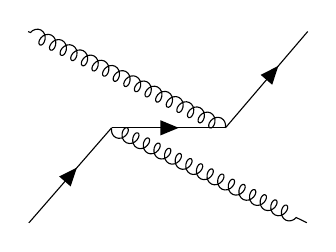
\begin{tikzpicture}[xscale=.95, yscale=1.]
  \begin{feynman}
    \diagram [horizontal=a to b] {
      i1 %[particle=\(Q\)]
      -- [fermion] a
      -- [draw=none] f1,% [particle=\(g\)],
      a -- [fermion] b,
      i2 %[particle=\(Q\)]
      -- [anti fermion] b
      -- [draw=none] f2,% [particle=\(g\)],
    };
    \diagram* {
      (a) -- [gluon] (f2),
      (b) -- [gluon] (f1),
    };
  \end{feynman}
\end{tikzpicture}
\feynmandiagram [xscale=1.2, yscale=.8, horizontal=p2 to p4] {
  p2 [particle=$g$]-- [gluon] b -- [gluon] p4 [particle=$g$],
  a -- [gluon] b,
  p1 [particle=$Q$] -- [fermion] a -- [fermion] p3 [particle=$Q$],
};
\feynmandiagram [xscale=1.2, yscale=.8, horizontal=p1 to p3] {
  p2 [particle=$q$] -- [fermion, edge label=$p_2$] a -- [fermion, edge label=$p_4$] p4 [particle=$q$],
  a -- [gluon, momentum=$q$] b,
  p1 [particle=$Q$] -- [fermion, edge label=$p_1$] b -- [fermion, edge label=$p_3$] p3 [particle=$Q$],
};
\caption{Elastic processes. The first three diagrams contribute to heavy quark (Q) - gluon (g) scattering, the last one contributes to a light (anti-)quark (q) scattering. Intermediate propagators are screened by a Debye mass in case of soft divergence.}\label{plots:feyn-elastic}
\end{figure}

\begin{figure}
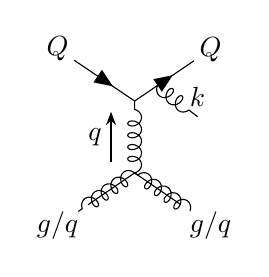
\begin{tikzpicture}
  \begin{feynman}
    \diagram [xscale=0.8, yscale=.6, vertical=a to b] {     
      i2 [particle=\(g/q\)]
        -- [gluon] b
        -- [gluon] f2 [particle=\(g/q\)]],
      b -- [gluon, momentum=$q$] a,
      i1 [particle=\(Q\)]
        -- [fermion] a
        -- [fermion] f1 [particle=\(Q\)],
    };
    \vertex [below right=.2 cm and .8 cm of a, label=\(k\)] (r);
    \draw [gluon] ($(a)!0.3!(f1)$) -- (r);
    \draw  (i2)--(b);
     \draw  (b)--(f2);
  \end{feynman}
\end{tikzpicture}
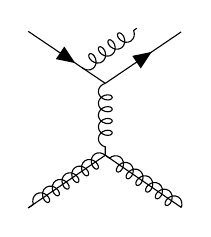
\begin{tikzpicture}
  \begin{feynman}
    \diagram [xscale=0.8, yscale=0.6, vertical=a to b] {     
      i2  -- [gluon] b
        -- [gluon] f2,
      a -- [gluon] b,
      i1 -- [fermion] a
        -- [fermion] f1,
    };
    \vertex [above right=.7 cm and .4 cm of a] (r);
    \draw [gluon] ($(i1)!0.7!(a)$) -- (r);
    \draw  (i2)--(b);
     \draw  (b)--(f2);
  \end{feynman}
\end{tikzpicture}
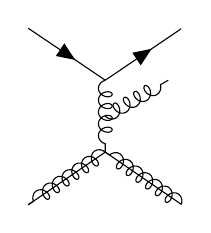
\begin{tikzpicture}
  \begin{feynman}
    \diagram [xscale=0.8, yscale=.6, vertical=a to b] {     
      i2 %[particle=\(g\)]
        -- [gluon] b
        -- [gluon] f2, %[particle=\(g\)]],
      a -- [gluon] b,
      i1 %[particle=\(Q\)]
        -- [fermion] a
        -- [fermion] f1, %[particle=\(Q\)],
    };
    \vertex [below right=.0 cm and .8 cm of a] (r);
    \draw [gluon] ($(a)!0.5!(b)$) -- (r);
    \draw  (i2)--(b);
     \draw  (b)--(f2);
  \end{feynman}
\end{tikzpicture}
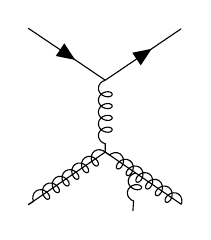
\begin{tikzpicture}
  \begin{feynman}
    \diagram [xscale=0.8, yscale=.6, vertical=a to b] {     
      i2 %[particle=\(g\)]
        -- [gluon] b
        -- [gluon] f2, %[particle=\(g\)]],
      a -- [gluon] b,
      i1 %[particle=\(Q\)]
        -- [fermion] a
        -- [fermion] f1, %[particle=\(Q\)],
    };
    \vertex [below right=.75 cm and .35 cm of b] (r);
    \draw [gluon] ($(i2)!0.6!(b)$) -- (r);
    \draw  (i2)--(b);
     \draw  (b)--(f2);
  \end{feynman}
\end{tikzpicture}
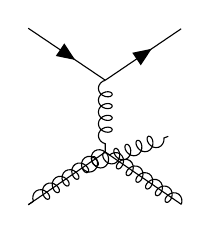
\begin{tikzpicture}
  \begin{feynman}
    \diagram [xscale=0.8, yscale=.6, vertical=a to b] {     
      i2 %[particle=\(g\)]
        -- [gluon] b
        -- [gluon] f2, %[particle=\(g\)]],
      a -- [gluon] b,
      i1 %[particle=\(Q\)]
        -- [fermion] a
        -- [fermion] f1, %[particle=\(Q\)],
    };
    \vertex [above right=.2 cm and .8 cm of b] (r);
    \draw [gluon] ($(b)!0.3!(f2)$) -- (r);
    \draw  (i2)--(b);
     \draw  (b)--(f2);
  \end{feynman}
\end{tikzpicture}
\caption{Inelastic process. Heavy quark collide with a meidum light (anti-)quark or gluon and radiates an additional gluon.}\label{plots:feyn-inelastic}
\end{figure}

\subsection{Diffusion component}
The diffusive motion of heavy quarks are solved in Langevin equations in terms of drag and diffusion.
The Langevin equations in the Ito scheme are,
\begin{eqnarray}
\Delta \vec{x}_i &=& \frac{\vec{p}_i}{E} \Delta t	\\
\Delta \vec{p}_i &=& -\Gamma \vec{p}_i \Delta t + \Delta t \vec{\xi}
\end{eqnarray}
The first equation is the spatial transport.
IN the second equation, momentum of heavy quarks are changed by a drag term with coefficient $\Gamma$ and a thermal random force $\vec{\xi}$. 
The random force has zero mean and the covariance structure:
\begin{eqnarray}
\langle \xi_i \xi_j \rangle = \frac{1}{\Delta t}\left(\Kpara \frac{p_i p_j}{p^2} + \Kperp \left(\delta_{ij} - \frac{p_i p_j}{p^2}\right) \right)
\end{eqnarray}
In this study, we assume the diffusion component is isotropic $\Kpara=\Kperp=\kappa$.
The drag coefficient $\Gamma$ and the momentum diffusion coefficient $\kappa$ need to satisfy the Einstein relation in Ito scheme to guarantee reaching the correct thermal equilibrium at large time,
\begin{eqnarray}
\Gamma &=& \frac{\kappa}{2TE} - \frac{d\kappa}{dp^2}
\end{eqnarray}
We choose momentum diffusion $\kappa$ as the independent variable in our parametrization.
If temperature is the only scale in the problem, we expect $\kappa$ to scale as $T^3$.
Additional, we consider the possibility of non-perturbative contribution to the diffusion component, which only happens at low energy and low temperature and we arrive at this simple ansatz,
\begin{eqnarray}
\frac{\kappa}{T^3} = \kappa_D\left(x_D + (1-x_D)\frac{[1\textrm{ GeV}]^2}{ET}\right)
\end{eqnarray}

\section{Tests in a static medium}\label{section:test}
\begin{figure}
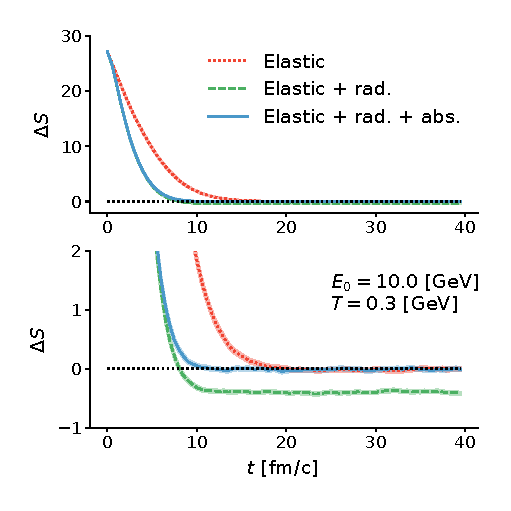
\includegraphics[width=\columnwidth]{thermalization.pdf}
\caption{The approach to thermalization of the linear Boltzmann equation with elastic processes only (red dot), elastic with radiation processes (green dashed), and elastic with both radaition and absorption processes (blue solid). The static medium has a temperature $T = 0.4$ GeV. $10^4$ heavy quarks are initialized with $E = 10$ GeV at $t = 0$.}\label{plots:thermalization}
\end{figure}

Before coupling the heavy quark transport model to a realistic medium, we study the behavior of the model in a static medium, i.e., the medium is at rest with a fixed temperature.
We first show our implementation indeed respect detailed balance and reaches thermal equilibrium.
To quantify the approaching to thermal equilibrium of an ensemble of $N$ heavy quarks in a medium with temperature $T_0$, we define the following quantity,
\begin{eqnarray}
\Delta S = \frac{1}{N}\sum_{i=1}^{N} \ln f_0(E_i) - \frac{\int f_0(p)\ln f_0(E) dp^3}{\int f_0(p) dp^3}
\end{eqnarray}
$f_0 \propto \exp(-E/T_0)$ is the Boltzmann-J\"uttner distribution function at temperature $T_0$. 
The second term is the entropy at this temperature, while the first term takes the heavy quarks ensemble average of $\ln f_0(E)$.
This difference $\Delta S$ defines a ``distance" from the heavy quark ensemble to the thermal distribution, and it vanishes when heavy quark ensemble is thermalized.
If the ensemble distribution $f$ is not far from thermal equilibrium and can be characterized by an effective temperature $T_{\textrm{eff}}$ so that $f(E)\sim \exp(-E/T_{\textrm{eff}})$, then this ``distance" measures,
\begin{eqnarray}
\nonumber
\Delta S &\sim& \frac{1}{T_0}\int  e^{-E/T_{\textrm{eff}}} E dp^3 - \frac{1}{T_0}\int e^{-E/T_0} E dp^3 \\
&=& \frac{T_\textrm{eff}-T_0}{T_0}
\end{eqnarray}
the fraction deviation of the effective temperature from the temperature of the thermal bath.
Figure \ref{plots:thermalization} shows the time-evolution of $\Delta S$ of $10^4$ charm quarks inside thermal bath $T=0.4$ GeV with initial energy $E_0 = 10$ GeV.
With elastic process only, the system thermalizes after about $50$ fm/$c$.
If we further turn on radiation process, the system reaches equilibrium faster, but it is wrong equilibrium.
The effective temperature is lower than the temperature of the thermal bath.
This is the consequence of breaking detailed balance if model only has radiation process.
Finally, we showed the case with both radiation and absorption turned on, the correct equilibrium is reached at $t\sim 20$ fm/c.
The absorption processes only make a notable difference when the system is not far from equilibrium ($\Delta S < 1$), which is expected from our previous argument.
\begin{figure}
\includegraphics[width=\columnwidth]{Eloss.pdf}
\caption{}\label{plots:dEE}
\end{figure}

\begin{figure}
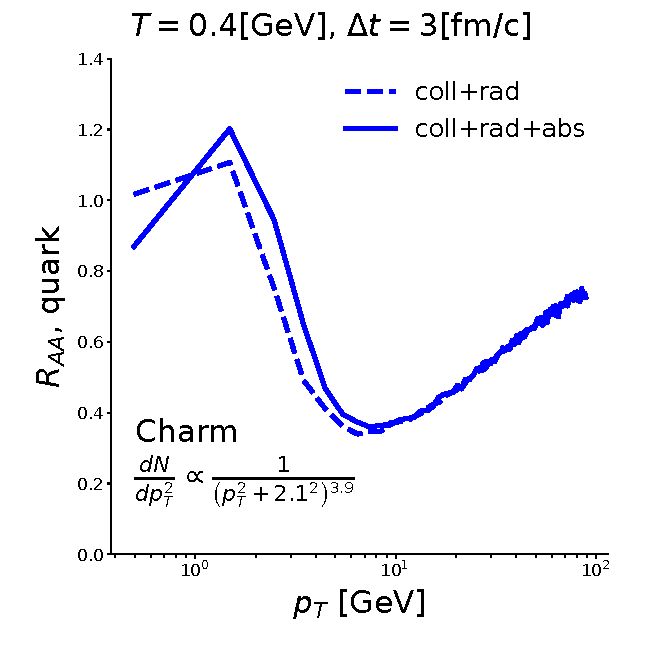
\includegraphics[width=\columnwidth]{BoxRaa.pdf}
\caption{}\label{plots:BoxRaa}
\end{figure}
From the rate equation \ref{eq:rate} one can actually calculate the heavy quark energy loss per unit time by inserting $\Delta E$ into the integration of differential rates.
This is straightforward for elastic processes, but because the rates of inelastic processes depend on history, a meaningful energy loss can only be obtained from an actually simulation.
And as we will see, this history dependence causes a non-trivial path length (medium size $L$) dependent energy loss.
In the first row of Figure \ref{plots:dEE}, we plot energy loss fraction $\Delta E/E$ for elastic process (left) and inelastic process (right) as function of $E$ for path length $5$ fm and temperature $T=0.2$ and $0.4$  GeV.
The elastic energy loss fraction is large at intermediate energy and decreases towards small and large energies.
At sufficient low energy, heavy quarks starts to gain energy from the medium on average that manifests as $\Delta E/E < 0$.
For the case of inelastic energy loss, we study the effect of gluon absorption process by comparing $\Delta E/E$ with only radiation process (lines) to $\Delta E/E$ with both gluon radiation and absorption (lines with symbols).
As expected, we find that gluon absorption process only affects energy loss significantly at low energy high temperature.
At sufficient low energy, gluon absorption process allow the heavy quark to gain energy from the medium through inelastic channel which is key to thermalization.

In the second row of Figure \ref{plots:dEE}, we show the path length dependence of the two energy loss mechanism.
Here, we plot the energy loss fraction per unit length, with length measured in units of inverse temperature.
The key observation is that elastic energy loss increases linearly with path length but inelastic energy loss increases non-linearly for small path length and then transits to a linear increase at large path length. 
The non-linear $L-$dependent energy loss is actually a characteristic behavior of the coherence effect in a finite length medium. 
In our effective implementation of the LPM effect, this arises because the gluon radiation with $\tau_f \sim k/T^2 \gg L$ is suppressed.
Therefore for a thin medium, the phase space for gluon radiation is very restricted $k < LT^2$, which is the typical amount of energy heavy quark loses per radiation.
Multiplied by an estimated of number of collisions $N \propto LT$ the inelastic energy loss scales as $\Delta E \sim L^2T^3$.
On the other hand, for a long path length, a energy heavy quark could have radiated gluons multiple times $N \propto L/\tau_f$ and each time the radiation carries off a typical amount of energy. 
In this region, the inelastic energy loss rises linearly with $L$.
What we see in the simulation is a behavior that interpolates between these two limits.

Finally, we calculate the $R_{AA}$ of charm and bottom quark in a static medium $T=0.4$ GeV after evolving for $3$ fm/c.
The initial spectra of the charm and bottom are parametrized as the one showed in [cite].
This simplified setup is far from realistic to compare to experimental measured $R_{AA}$, but is intended for comparison with other models.
In Figure \ref{plots:BoxRaa} we showed both $R_{AA}$ of charm and bottom with or without turning on the gluon absorption process. 
Again, we see that the absorption process only affects observables for relatively low momentum $p_T < 10$ GeV.
The mass plays an important role in the intermediate $p_T$ region, where a clear separation between charm and bottom $R_{AA}$.
The mass effect is neither important at high energy where $p_T$ is the only relevant scale or low $p_T$ when $M (\gg p_T, T)$ becomes the only relevant scale. 

\section{Calibration of the model at LHC using Bayesian analysis}\label{section:calibration}
In this section, we couple the heavy quark transport model in a realistic event-by-event medium evolution and extract the transport model parameters  from a Bayesian model-to-data comparison.
The medium evolution model consists of multiple stages,
\begin{itemize}
\item[1.] The TRENTo model generates event-by-event initial condition at time $\tau = 0^+$. 
\item[2.] A collision-less Boltzmann equation (freestreaming) models the pre-equilibrium stage before the onset of hydrodyanmics expansion.
\item[3.] The 2+1D relativistic viscous hydrodynamics evolves the QGP with a lattice equation of state.
\item[4.] Finally, hadrons sampled from hydrodynamic energy momentum tensors rescatter and decay in the Ultra-Relativistic Quantum Molecular Dynamics (UrQMD) model.
\end{itemize}
The parameters of this bulk event generator (public available) have already been calibrated to reproduce a vast of bulk observables at the LHC energies, providing a description of bulk evolution with unprecedented precision.
On the heavy quark transport side, we initialize heavy quark ensembles with the momenta sampled from FONLL calculation using either EPPS or nCTEQ15np nuclear parton distribution function. 
The position of the hard production vertices at $\tau = 0^+$ are sampled from TRENTo binary collision density to correlate with hot-spots of  underlying event. 
During the pre-equilibrium stage the heavy quark should already start to interact with medium.
However, the system is still far from both kinetic and chemical equilibrium.
To get a handle on the effect of pre-equilibrium energy loss on heavy quark, we choose to define the meidum flow velocities and energy density from the pre-equilibrium energy-momentum tensor by Landau macthing and further convert the energy density to a temperature using a 3-flavor conformal QCD equation of state. 
Heavy quarks are allowed to loose energy starting from a tunable energy-loss onset time $0.1\textrm{ fm/c} < \tau_0 < \tau_{\textrm{fs}}$. 
With a small $\tau_0$, this correspond to a fast generate of degrees of freedom in the medium that can collide with heavy quarks at very early time, and with a large $\tau_0$ the pre-equilibrium effects gradually turns off.
This is of course a very simple and crude setup, we are looking for more sophisticated models to treat pre-equilibrium stage energy loss.
During the hydrodynamic expansion stage, the time evolution of the flow velocities and temperature are provided by the 2+1D viscous hydro dynamics with boost-invariance in the beam direction.
The heavy quarks then hadronize in a sudden-approximation at $T = 154$ MeV.
Both the fragmentation and the recombination mechanisms are included. 
The bottomed mesons cease to interact at this point in our model, but the charmed mesons are included in the UrQMD afterburner with $\pi$-D and $\rho$-D cross-sections.

We summarize the model parameters in the heavy flavor sector,
\begin{itemize}
\item[1.] $\tau_0$ the time at which heavy quark energy loss starts, varies between $0.1$ fm/c to $1.0$ fm/c.
\item[2.] $\mu$, the medium energy scale parameter that appears in the running coupling constant of the scattering component, varies from $\pi/3$ to $4\pi$.
\item[3.] $\kappa_D$, the strength of momentum diffusion at $ET = 1 \textrm{GeV}^2$, range from $0$ to $8$.
\item[4.] $x_D$, the fraction of the momentum diffusion that is energy independent, ranges from $0$ to $1$.
\end{itemize}
An additional variable factor is the nuclear parton distribution function.
The nuclear PDF often comes with large uncertainty in the shadowing region which is relevant a the LHC energies.
However, it is hard to parametrize its uncertainty in our study as other parameters.
Instead, we choose to use the center values of two different sets of nuclear PDF, namely the EPPS set and the nCTEQ16np set and perform calibrations using both to demonstrate the sensitivity of the parameter extraction on the nuclear PDF uncertainty.
The difference between the two can to some extent reflects the uncertainties in our understanding of the nuclear shadowing effects.

The calibration of multiple parameters of a computationally time-consuming model is solved by the Bayesian model-to-data comparison framework developed in our group.
Here, we briefly introduce the idea of this Bayesian technique and key terminologies to be used later.
For more details, one can to the thesis work [] for an exhaustive study and to previous works [] for applications to bulk evolution and to heavy quark sector using an radiation improved Langevin transport model.
Given a model whose prediction ${\bf y}$ depends on a vector of input parameters ${\bf p}$ and the experimental data ${\bf y}_\textrm{exp}$, 
the probability distribution of the {\it true} model parameters ${\bf p^*}$ is given by the Baye's theorem, 
\begin{eqnarray}\label{eq:Bayes}
\textrm{Posterior}({\bf p^*}|{\bf y}_\textrm{exp}, M) &\propto& \textrm{Likelihood}({\bf y}_\textrm{exp}|{\bf p^*}, M) \nonumber \\ &\times& \textrm{Prior}({\bf p^*}).
\end{eqnarray}
The posterior probability distribution of the ${\bf p^*}$ given certain model $M$ and data, equals the probability $L$ of observing data given model and parameters ${\bf p^*}$, called likelihood function, times a prior belief on the distribution of ${\bf p^*}$.
The likelihood function is often defined in a Gaussian form in terms of the difference between model calculation and experimental data and a covariance matrix that encodes experimental and theory uncertainty,
\begin{eqnarray}\label{eq:likelihood}
\ln(L) &=& -\frac{1}{2}({\bf y}-{\bf y}_{\textrm{exp}})^T\Sigma^{-1} ({\bf y}-{\bf y}_{\textrm{exp}})\nonumber\\ 
		&-&\frac{d}{2}\ln(2\pi)-\frac{1}{2}\ln|\Sigma|.
\end{eqnarray}
Once we have the ability to evaluate model output given arbitrary parameters within a reasonable range, the information of parameters constrained by data follows from Equations \ref{eq:Bayes} and \ref{eq:likelihood}.
And this high-dimensional posterior probability distribution function can be studied by a Markov-chain Monte Carlo (MCMC) sampling procedure.
The difficulty for applying this directly event-by-event heavy-ion collision simulation are that the model itself is computationally heavy and that one needs to averaged over a lot of random events to get statistical error of calculation under control.
Therefore, it is unpractical to evaluate the model output at arbitrary points in the parameter space in during the MCMC sampling.
The solution is to use advanced sampling technique to sample O(100) design parameter sets in the parameter space and calculate the corresponding model outputs.
Then, use a Gaussian process emulator to fast interpolate the model outputs with estimated uncertainty at arbitrary point in the parameter space.
\begin{center}
\begin{table}[h]
\caption{ALICE dataset}\label{table:ALICE-obs} 
\begin{tabularx}{\columnwidth}{Xl}
\hline 
 Observables & Centrality \\ 
\hline 
D-meson $v_2$ & 30-50\% \\ 
Event-engineered D-meson $v_2$ & 30-50\% \\ 
D-meson $R_{AA}$ & 0-10\% 30-50\% 50-80\% \\
\hline 
\end{tabularx}
\end{table}
\begin{table}[h]
\caption{CMS dataset}\label{table:CMS-obs} 
\begin{tabularx}{\columnwidth}{Xl}
\hline 
Observables & Centrality \\ 
\hline 
D${}^0$-meson $v_2$ & 0-10\%, 10-30\%, 30-50\% \\ 
D${}^0$-meson $R_{AA}$ & 0-10\%, 0-100\% \\ 
B${}^{\pm}$-meson $R_{AA}$ & 0-100\% \\ 
\hline 
\end{tabularx}
\end{table}
\end{center}

In our study, we sampled 80 design points in the four dimensional parameter space $(\tau_0, \mu, \kappa_D, x_D)$.
For each parameter set, we ran 4000 minimum biased event.
Each event propagates an ensemble of $4\times 10^4$ charm quarks and $10^4$ bottom quarks as described above.
The centrality is defined by mid-rapidity charged particle yield and the same kinematic cuts as experimental measures are applied to the calculation of heavy flavor observables.
All these observables are measured at 5.02 TeV in Pb+Pb, as listed in Table \ref{table:ALICE-obs} and \ref{table:CMS-obs} and here are a few remarks on our choice.
Most of these data are for D-meson and in additional to the $R_{AA}$ and $v_2$ that one usually fit to. 
We also compare to the event-engineered D-meson flow being measured at ALICE.
The idea of the event-engineering is to subdivide events in a certain centrality according to the magnitude of charged particle $q$-vector, in this case,
\begin{eqnarray}
|q_2|^2 = \frac{\left(\sum_{i=1}^{M} \cos(2\phi) \right)^2+ \left(\sum_{i=1}^{M} \sin(2\phi) \right)^2}{M}
\end{eqnarray}.
The D-meson $v_2$ is measured for those events with $20\%$ highest $q_2$ and events with $60\%$ lowest $q_2$.
It is found that D-meson flow is strongly correlated with this measure of bulk collectivity.
This event-engineering procedure necessitates a full event-by-event study and may be sensitive to the interplay between heavy quark energy loss and initial condition fluctuation, so we include it as an observable to calibrate on.
Finally to investigate if the model predicts the correct mass-dependence, we include recent CMS measurements of $B^{\pm}$-meson $R_{AA}$, although the data has a large uncertainty which decreases its importance in the likelihood function.
\begin{figure*}
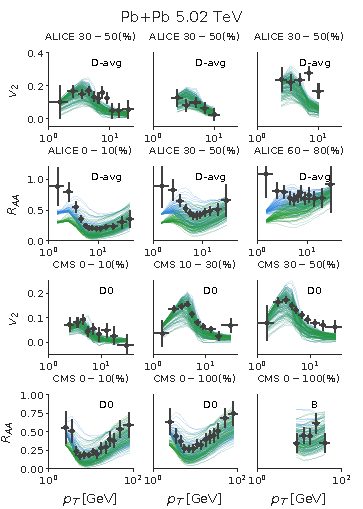
\includegraphics[width=.49\textwidth]{observables_design.pdf}
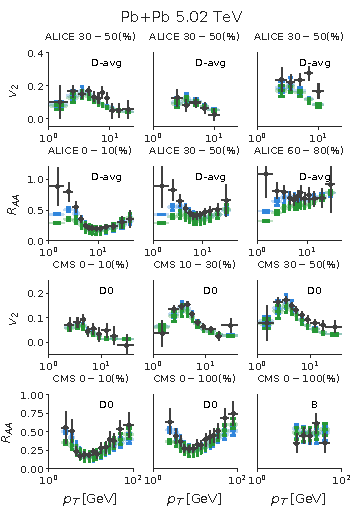
\includegraphics[width=.49\textwidth]{observables_posterior.pdf}
\caption{...}\label{plots:deisgn_posterior_obs}
\end{figure*}

On the left of Figure \ref{plots:deisgn_posterior_obs}, we show the prior range of our calculations for each of the listed observables. 
We use different colors to distinguish calculations using EPPS (blue) and
nCTEQnp (green) nuclear PDF.
The calculated $R_{AA}$ at high transverse momenta and $v_2$ at low transverse momenta are spread enough to cover the experimental data.
We noticed that our model are always below data points for the very low-$p_T$ ALICE $R_{AA}$ and 30-50\% high-$p_T$ CMS $v_2$.
This could be limitations of our model, such as the need of more sophisticated implementation of LPM effect and more accurate calculation of low-$p_T$ charm quark production. 
Plots on the right of Figure \ref{plots:deisgn_posterior_obs} show the posterior distribution of the observables from model emulators.
The calibrated model displays a very good overall fit to all the observables except for the limitations pointed out above.
The use of different nuclear PDF makes negligible difference for azimuthal anisotropy, but does affect the shape of $R_{AA}$.
Calculations with EPPS nuclear PDF works very well for $p_T < 50$ GeV, while calculations with nCTEQnp does better at describing very high $p_T$ CMS data.
The calculated event-engineered flow also shows strong correlation with charged particle $|q_2|$ and describes the lowest 60\% $q_2$ bin very well.
For the highest 20\% $q_2$ bin, model posterior is consistent with measurements below $5$ GeV and underestimates the data at higher $p_T$ bins.

\begin{figure}
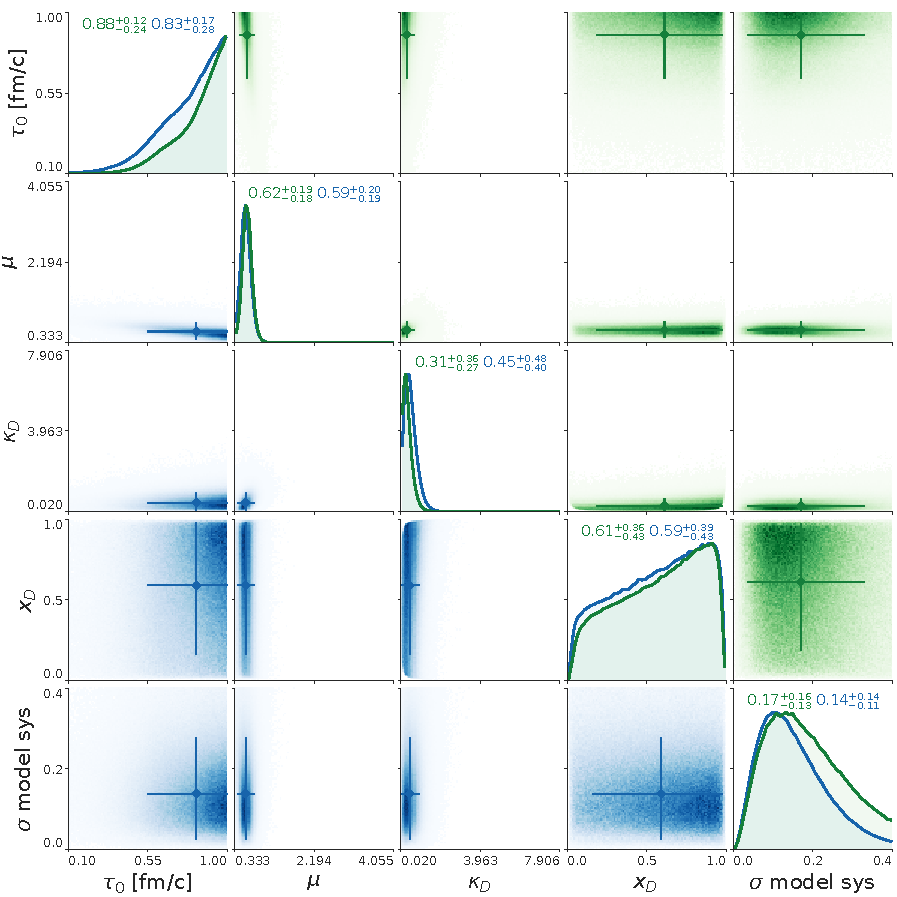
\includegraphics[width=.5\textwidth]{posterior.pdf}
\caption{...}\label{plots:posterior}
\end{figure}

The posterior probability distribution of the parameters are marginalized to single parameter distribution (diagonal) and two-parameter joint distribution (off-diagonal) in Figure \ref{plots:posterior}.
The lower off-diagonal plots and blue lines in the diagonal plots correspond to the extraction using EPPS nuclear PDF, and the off-diagonal plots abd green lines in the diagonal plots uses nCTEQ15np nuclear PDF.
Despite the difference in $R_{AA}$ when different nuclear PDFs are used, the extracted probability distribution of parameters are similar.
To describe LHC data, the model prefers a late onset of medium induced energy loss and a medium energy scale roughly around $0.6\pi T$, which means the largest coupling constant at certain temperature is $\alpha_s \sim \alpha_s(1.8T)$.
A small but finite amount of momentum diffusion at $ET=1\textrm{ GeV}^2$ is preferred for the diffusion component.
The smallness of this number is expected because most of the interaction are already taken account by the scattering component with relatively large coupling constant (a small medium scale).
But this study is not sensitive to the energy / temperature dependence of the diffusion component other than the regular $T^3$ scaling of the momentum diffusion constant.   

To define the total momentum broadening parameter of a heavy quark,
we combine the contribution from both elastic scatterings and the diffusion component,
\begin{eqnarray}\label{eq:qhat}
\frac{\hat{q}}{T^3} &=& \frac{1}{T^3}\frac{d}{dt}\left\langle p_\perp^2 \right\rangle\\
\nonumber
 &=&  \kappa_D\left(x_D + (1-x_D)\frac{\textrm{GeV}^2}{ET}\right) + \frac{\hat{q}_{\textrm{el}}}{T^3}.
\end{eqnarray}
Where $\hat{q}_{\textrm{el}}$ is obtained by integrating the rate equation with transverse momentum transfer square.
We shall discuss the inclusion of inelastic process into the calculation $\hat{q}$ in section \ref{section:conclusion}.
Performing this calculation for many random parameter set samples drawn from the posterior distribution using either nuclear PDF, we estimate the posterior distribution of the functional $\hat{q}(E, T)$ constrained by data.
On the left of Figure \ref{plots:posterior_qhat}, we showed the 90\% credible region of $\hat{q}$ as function of temperature, fixing heavy quark momenta at $10$ GeV.
And the right panel the figure shows $\hat{q}$ as function of momenta at $T=0.35$ GeV.
Our formula is mass dependence and the charm quark $\hat{q}$ (region enclosed by thick red lines and slashes) is slightly different from the bottom quark $\hat{q}$ (region enclosed by thick blue lines).
Comparing to former work by Yingru et al (green shaded region), who used an improved Langevin model to extract charm quark transport properties at the LHC, the present result is consistent but hits the lower half of the 90\% credible region of the previous extraction.
\begin{figure}
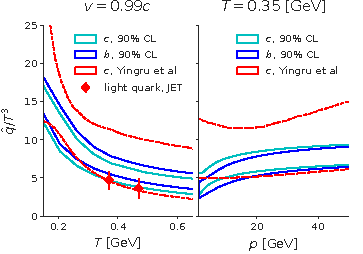
\includegraphics[width=\columnwidth]{qhat_p_T.pdf}
\caption{...}\label{plots:posterior_qhat}
\end{figure}
There is also a heavy quark spatial diffusion constant $D_s$ often defined in the limit of $p\ll M$.
It is related to the momentum diffusion parameter by,
\begin{eqnarray}
2\pi T D_s = \frac{8\pi T^3}{\hat{q}(p\rightarrow 0, T)}
\end{eqnarray}
In figure \ref{plots:posterior_Ds}, we plotted the 90\% credible region of both charm (region enclosed by red thick lines and slashes) and bottom (region enclosed by blue tick lines) quark spatial diffusion constant as function of $T/T_c$.
The results of this work is systematically higher than the extraction from the former work (green shaded region).
The spatial diffusion constant has been calculated from first principal using lattice QCD.
There are two calculations available, a calculation that assumes static heavy quark (blue symbols with higher values and larger errorbars) and the other calculation for realistic charm quark (red symbols with lower values and smaller errorbars).
Our posterior in $D_s$ with diffusion component and only elastic channel contribution agrees with the static heavy quark limit lattice evaluation.
Again, the effect of including inelastic channel in $D_s$ is discussed in the last section.

To summarize this section, we perform a Bayesian calibration on the model parameters. 
We found a general agreement to the data.
The extracted parameters indicate a late onset of medium induced heavy quark energy loss and a small by finite diffusion component is preferred.
The posterior transport coefficient $\hat{q}$ and spatial diffusion constant $D_s$ is calculated and $D_s$ agrees with lattice calculation in the static heavy quark limit. 

\begin{figure}
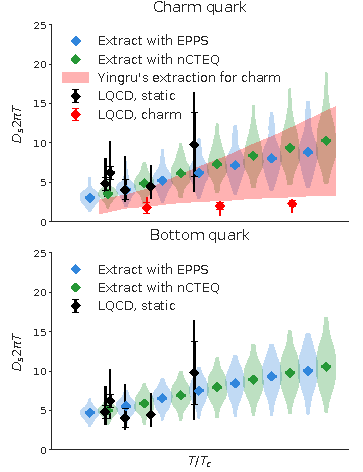
\includegraphics[width=\columnwidth]{Ds_posterior.pdf}
\caption{...}\label{plots:posterior_Ds}
\end{figure}

\section{Prediction}\label{section:prediction}
We can apply the calibrated model to predict for novel observables.
\subsection{D-meson $v_3$, and B-meson $v_n$}
\subsection{D-meson $v_1$}
D-meson $v_1$ should be vanishing at mid-rapidity if one measures it with respect to an estimated reaction plane.
But we can correlate $Q_1$ with charged particle $q_3$ to get a non-zero signal at mid-rapidity.
\begin{eqnarray}
v_1 = \left\langle \frac{\Re\{q_3 Q_1^*\}}{mM} \right\rangle
\end{eqnarray}
This is because when $q_3$ is non-zero, the direction of $q_3$ defines a plane to which the medium evolution is not reflection symmetric and this asymmetry should cause heavy quarks to loose energy differently depending moving along or against the direction of $q_3$.
Since $q_3$ originates from the triangular initial state fluctuation, a finite signal would be another indicator of D-meson energy loss coupling to initial condition fluctuations and collectivity of bulk evolution.
Here we showed the resulting $v_1$


\section{Discussion and Conclusion}\label{section:conclusion}
Before summarizing this work, we want to discuss more on the definition of $\hat{q}$ in our model.
In Equation \ref{eq:qhat} for the scattering component, we used only the elastic processes to evaluate $\hat{q}$.
This is because we have an order-by-order definition of $\hat{q}$ in pQCD.
In fact, the inelastic processes also contributes a diffusion-like part, but is shown to be one order higher in $\alpha_s$, though it may not be numerically small in realistic case compared to leading order.
So in the sense of calculate a leading order transport coefficient, it is sufficient to use only elastic channels in Equation \ref{eq:qhat}, and this is also conceptually cleaner to compare with other pQCD based calculations.
For lattice calculations, the results do not rely on the expansion in $\alpha_s$.
In that case, to make a reasonable comparison with lattice transport coefficient, we should calculate $\hat{q}$ from the calibrated model including both elastic and inelastic processes in the scattering component.
Unfortunately, currently there is not any lattice calculation of $\hat{q}$ at finite heavy quark momentum.  
Lattice $D_s$ do exist with $p \ll M$, but such momenta are too small for our calculation with Gunion-Bertsch matrix-elements to be valid.
Even so, we would like to show the $\hat{q}$ and $D_s$ with a set of high likelihood parameters that includes the inelastic processes.
Just like the energy loss showed in Figure \ref{plots:dEE}, the transverse momentum broadening per unit time in the presence of inelastic processes is not a constant a thin static medium.
Therefore, we setup the Monte Carlo simulation for fixed energy heavy quarks and extract $\hat{q}$ only after the finite path length effect fades away. 
\begin{figure}
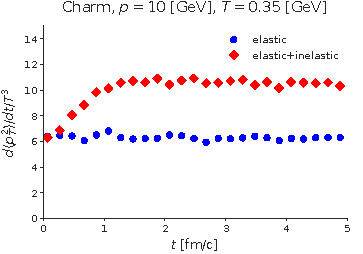
\includegraphics[width=0.5\textwidth]{qhat_full.pdf}
\caption{•}\label{plots:transport_full}
\end{figure}
Figure \ref{plots:transport_full} compares the $\hat{q}$ at $p=10$ GeV and $D_s$ before and after the elastic processes are turned on.
The calculation uses a high likelihood parameter set $\mu = 0.6, \kappa_D = 0.4$ and $x_D = 0.5$. 
We see a 30-40\% increase in $\hat{q}$ and similar amount of decrease in $D_s$ with the inelastic contribution.
\begin{appendices}
\section{Running coupling}
We use the leading order running coupling constant with three flavors of quark,
\begin{eqnarray}
\alpha_s(Q^2) = \frac{4\pi}{9 \ln\left(Q^2/\Lambda^2\right) }
\end{eqnarray}
The QCD scale is set at $\Lambda = 0.2$~GeV.
Inside a medium, the temperature $T$ defines the medium scale, it is used as a lower cutoff for $Q^2$ of all process, and the running coupling is actually,
\begin{eqnarray}
\alpha_s = \alpha_s(\max\{Q^2,(\mu T)^2\})
\end{eqnarray}
$\mu$ the only parameter we tuned in the scattering component of the hybrid model.
For elastic scattering, $Q^2$ is chosen as the momentum exchange squared for $s,t,u$ channel.
For the gluon emission / absorption vertex, we choose $Q^2 = k_\perp^2$.

\section{Evolution with both scattering and diffusion dynamics}
With a transport $\hat{T} = -v\cdot \partial_x$, a scattering $\hat{C}$, and a diffusion $\hat{D}$ operator in the hybrid transport equation,
\begin{eqnarray}
\frac{\partial f}{\partial t} = \left( \hat{T} + \hat{C} + \hat{D} \right) f
\end{eqnarray}
The formal solution is,
\begin{eqnarray}
f_{\Delta t} = e^{\int_0^{\Delta t}  \left( \hat{T} + \hat{C} + \hat{D} \right) dt}f_0
\end{eqnarray}
Assume the time variance of the medium are slow and decompose the joint operation into separate operations.
\begin{eqnarray}
e^{ \Delta t\left(\hat{T} +\hat{C} + \hat{D} \right)} &=&
\nonumber
e^{\Delta t \left(\hat{T} + \hat{D}\right) } e^{\Delta t \hat{C}}   e^{-\frac{\Delta t^2}{2} [\hat{T}+\hat{D}, \hat{C}]}\left(1+O(\Delta t^3)\right) \\
\nonumber
&=& \frac{1}{2}  \left\{
1+\Delta t \left( \hat{T}+\hat{D} \right), 1+\Delta t C
\right\} + O(\Delta t^3) 
\end{eqnarray}
The operator $1 + \Delta t ( \hat{T}  + \hat{D} )$ stands for a ``Diffusion" step in the simulation; the operator $1+\Delta t \hat{C}$ stands for a ``Scattering" step in the simulation. 
Therefore, we design the following simulation procedure.
\begin{itemize}
\item For each step, choose a $\Delta t$ in lab frame small enough that total scattering probability $P_c \ll 1$.
\item Determine the ordering of diffusion step and scattering step with 50-50\% chance
\item If diffusion operates before scattering.
\begin{itemize}
\item[Step 1.] $(t, x, p) \xrightarrow{\textrm{Diffusion}} (t+\Delta t, x', p^*)$.
\item[Step 2.] $(t+\Delta t, x', p^*) \xrightarrow{\textrm{Scattering}} (t+\Delta t, x', p')$.
\end{itemize}
\item If diffusion operates after scattering.
\begin{itemize}
\item[Step 1.] $(t, x, p) \xrightarrow{\textrm{Scattering}} (t, x, p^*)$.
\item[Step 2.] $(t, x, p^*)  \xrightarrow{\textrm{Diffusion}} (t+\Delta t, x', p')$.
\end{itemize}
\end{itemize}



\section{Calculation of $v_n\{2\}$ and $v_2\{EP\}$}
Cumulant method correlates a heavy meson with a light particle to estimate $v_n$. 
\begin{eqnarray}
v_n\{2\} &=& \frac{d_n\{2\}}{\sqrt{c_n\{2\}} } \\
d_n\{2\} &=& \left\langle \frac{\Re\{pQ^*\}}{mM} \right\rangle_{w = mM} \\
c_n\{2\} &=& \left\langle \frac{|Q|^2-M}{M(M-1)} \right\rangle_{w = M(M-1)}
\end{eqnarray}

\section{Matrix elements}
\label{appendix:matrix-element}
%\begin{widetext}
\begin{eqnarray}
\overline{|M_{22,Qq}|^2} &=& \frac{64\pi^2\alpha_s^2}{9} \frac{(M^2-u)^2 + (s-M^2)^2 + 2 M^2 t}{t^2}
\nonumber
\\
\overline{|M_{22,Qg}|^2} &=& \pi^2 \left\{
32\alpha_s^2 \frac{(s-M^2)(M^2-u)}{t^2} \right.
\nonumber
\\
&+&\frac{64}{9}\alpha_s^2 \frac{(s-M^2)(M^2-u)+2M^2(s+M^2)}{(s-M^2)^2} \nonumber
\\
&+&\frac{64}{9}\alpha_s^2 \frac{(s-M^2)(M^2-u)+2M^2(u+M^2)}{(M^2-u)^2} \nonumber
\\
&+& \frac{16}{9}\alpha_s^2 \frac{M^2(4M^2 - t)}{(M^2-u)(s-M^2)} 
\nonumber
\\
&+& 16 \alpha_s^2 \frac{(s-M^2)(M^2-u)+M^2(s-u)}{t(s-M^2)}
\nonumber
\\
&-& \left. 16 \alpha_s^2 \frac{(s-M^2)(M^2-u)-M^2(s-u)}{t(M^2u)}\right\}
\nonumber
\\
|M_{2\rightarrow 3}|^2 &=& |M_{2\rightarrow 2}|^2 48 \pi \alpha_s (1-\bar{x})^2
\nonumber
\\
&\times&\left(\frac{\vec{k}_\perp}{k_\perp^2 + x^2 M^2} + \frac{\vec{q}_\perp - \vec{k}_\perp}{(\vec{q}_\perp-\vec{k}_\perp)^2 + x^2 M^2}
\right)^2 
\end{eqnarray}
%\end{widetext}

\end{appendices}
\end{document}

